\documentclass[a4paper,12pt]{article}
\usepackage{amsmath,amsfonts,amsthm,amssymb}
\usepackage{physics}
\usepackage{setspace}
\usepackage{booktabs}
\usepackage{geometry}
\usepackage{graphicx}
\title{Coordinates and Linear Functions}
\author{}
\date{}
\doublespacing{}
\begin{document}
\maketitle

\section{Coordinates}
\subsection{Cartesian Plane}
The Cartesian Plane \(\left(\mathbb R^2\right)\) is a coordinate system for expressing the locations of points in the space with respect to the origin \(O(0,0)\).
The coordinates are expressed in the form of an ordered pair \((x,y)\),
where \(x\) is the x-coordinate and \(y\) is the y-coordinate.
The Cartesian Plane can also be thought as the Cartesian product of two real number lines,
such that \(\mathbb R\times\mathbb R=\mathbb R^2\).
\begin{center}
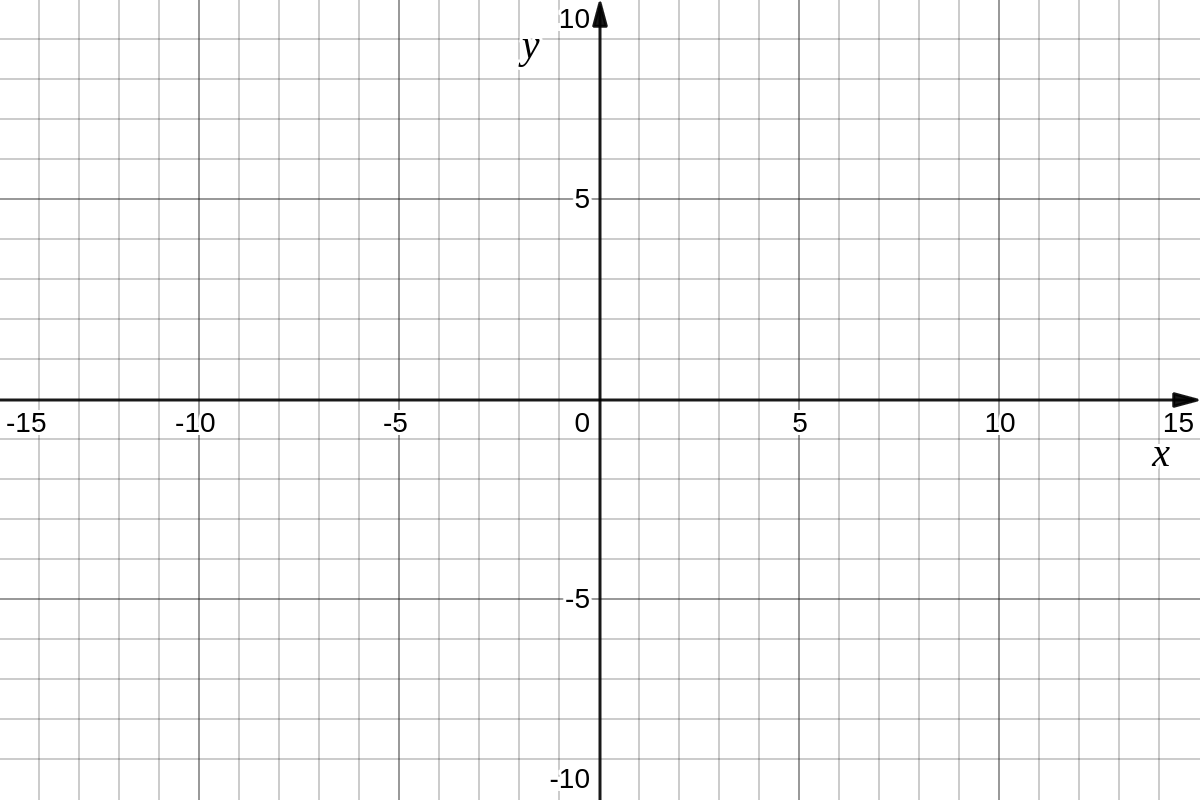
\includegraphics[width=.8\textwidth]{catesian.png}
\end{center}
\subsection{Example}
Plot and label the points \(A(4,5)\), \(B(-1,5)\) and \(C(-2,-3)\).\\
Plot and write down the coordinates of \(D\) such that \(ABCD\) is a parallelogram.
\begin{center}
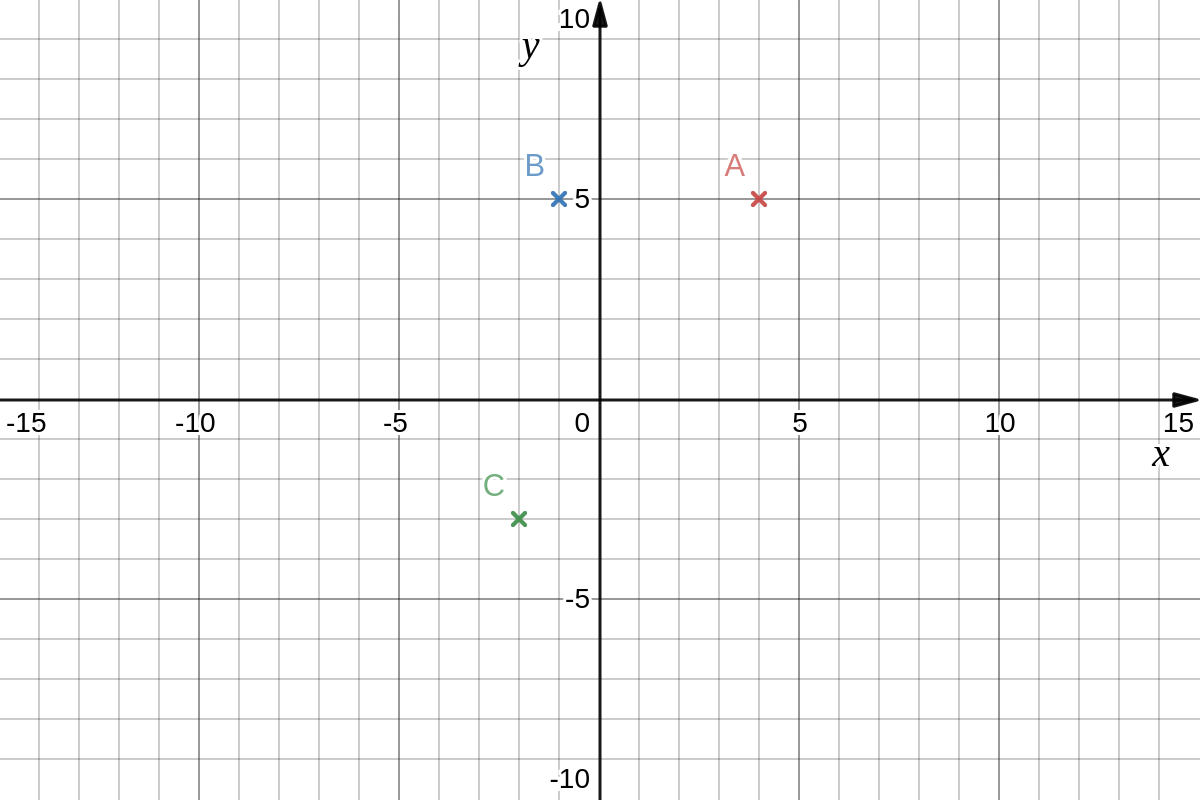
\includegraphics[width=.99\textwidth]{ex1cat.png}
\end{center}

\section{Functions}
A function is a rule that specifies one output given one input.
\subsection{Linear Functions}
A linear function has a rule that defines a straight line when \(y=f(x)\)
is drawn on a Cartesian plane.
\subsubsection{Example 1}
Let \(f\) be the number of maths problems you have done
and \(t\) be the amount of time you spent on doing maths problems in minutes.\\
It is given that you can do one question in 5 minutes. 
Write down the corresponding function which represents this rule.
\[\begin{array}{cccccc}
    \toprule
    t/\text{min}&5&10&15&20&25\\
    \midrule
    f(t)&1&2&3&4&5\\
    \bottomrule
\end{array}
\implies{}
f (t)=\frac15t\]
\begin{center}
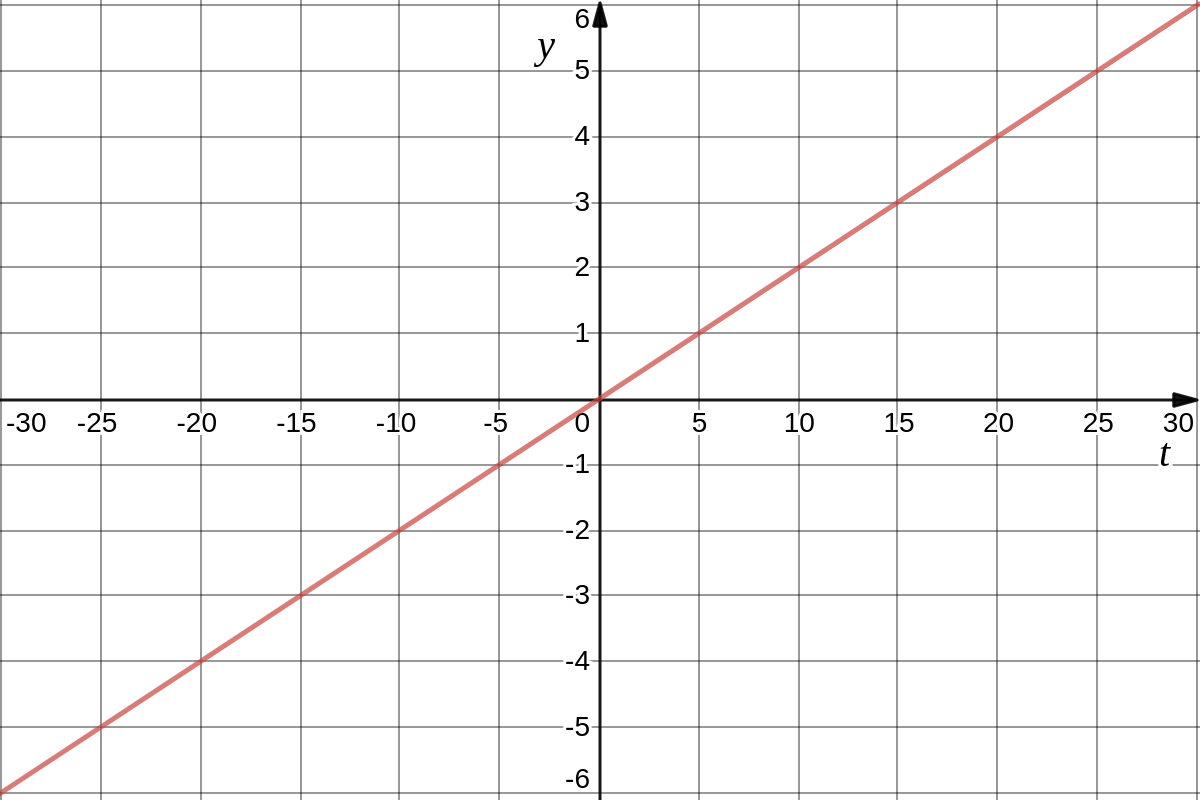
\includegraphics[width=.99\textwidth]{linear.png}
\end{center}
\subsection{Example 2}
The equation of a line is given as \(y=f(x)=2x+1\).\\
Does \((3,7)\) lie on the line?\\
Does \((4,10)\) lie on the line?\\
Given that \((a,9)\) lies on the line, find the value of \(a\).
\begin{center}
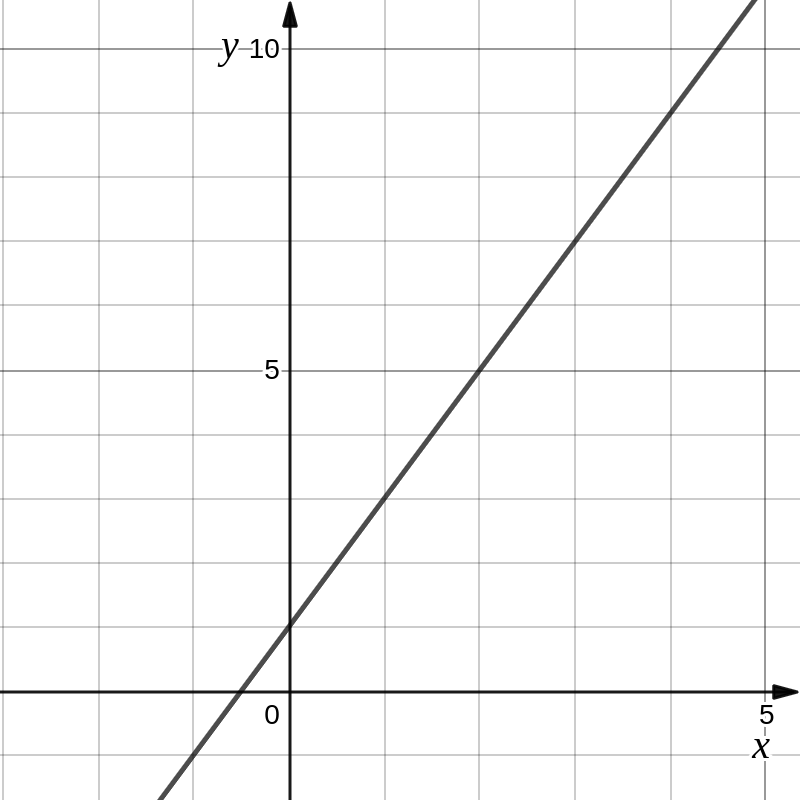
\includegraphics[width=.99\textwidth]{2x+1.png}
\end{center}

\section{Gradient}
Gradient determines the slope of a line, meaning how steep a line is.
One can imagine walking from the left to the right along the line,
the more difficult it is the walk, the greater the gradient it is.
Given that two points \((x_1,y_1)\) and \((x_2,y_2)\) lie on the line,
the gradient of the line is given as:
\[\text{gradient}=m=\frac{\Delta y}{\Delta x}=\frac{y_2-y_1}{x_2-x_1}\]
\begin{center}
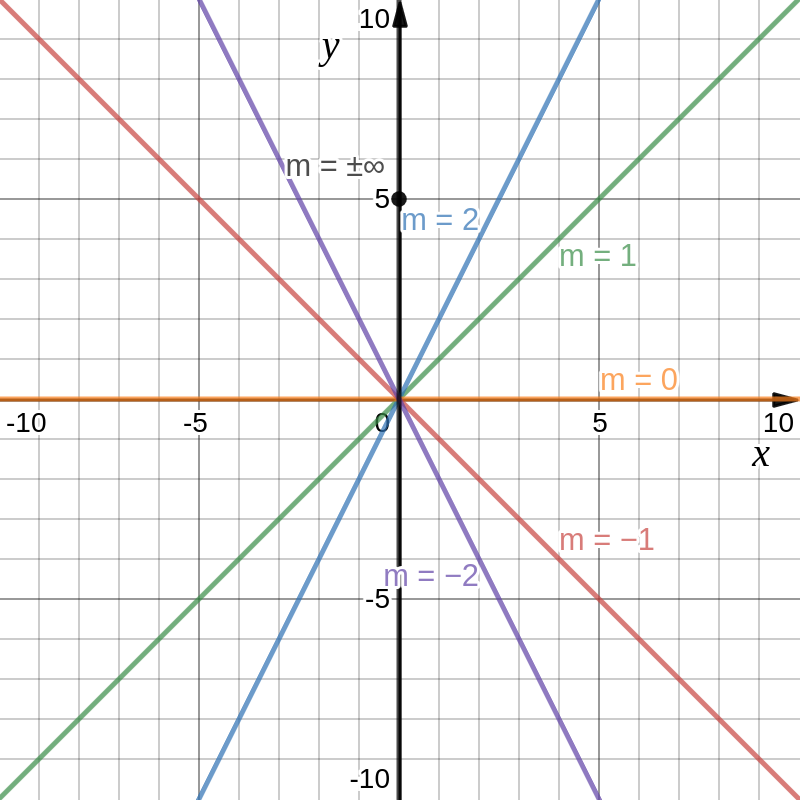
\includegraphics[width=.75\textwidth]{gradient.png}
\end{center}
\subsection{Example}
Compute the gradient of the line that passes through \((-2,5)\) and \((3,-8)\).

\section{Equation of Straight Lines}
The equation of a straight line, given its gradient \(m\) and 
y-intercept \(c\), is:
\[y=mx+c\]
\subsection{Example}
Find the gradients and y-intercepts of the following lines:
\[y=\frac32x+2\]
\[3x+4y=1\]
\newpage
\section{Plot of Linear Functions}
Complete the table and draw the graph of \(y=1-x\).
\[\begin{array}{cccc}
    \toprule
    x&-3&\quad\quad&3\\
    \midrule
    y&\quad\quad&1&\quad\quad\\
    \bottomrule
\end{array}\]
\begin{center}
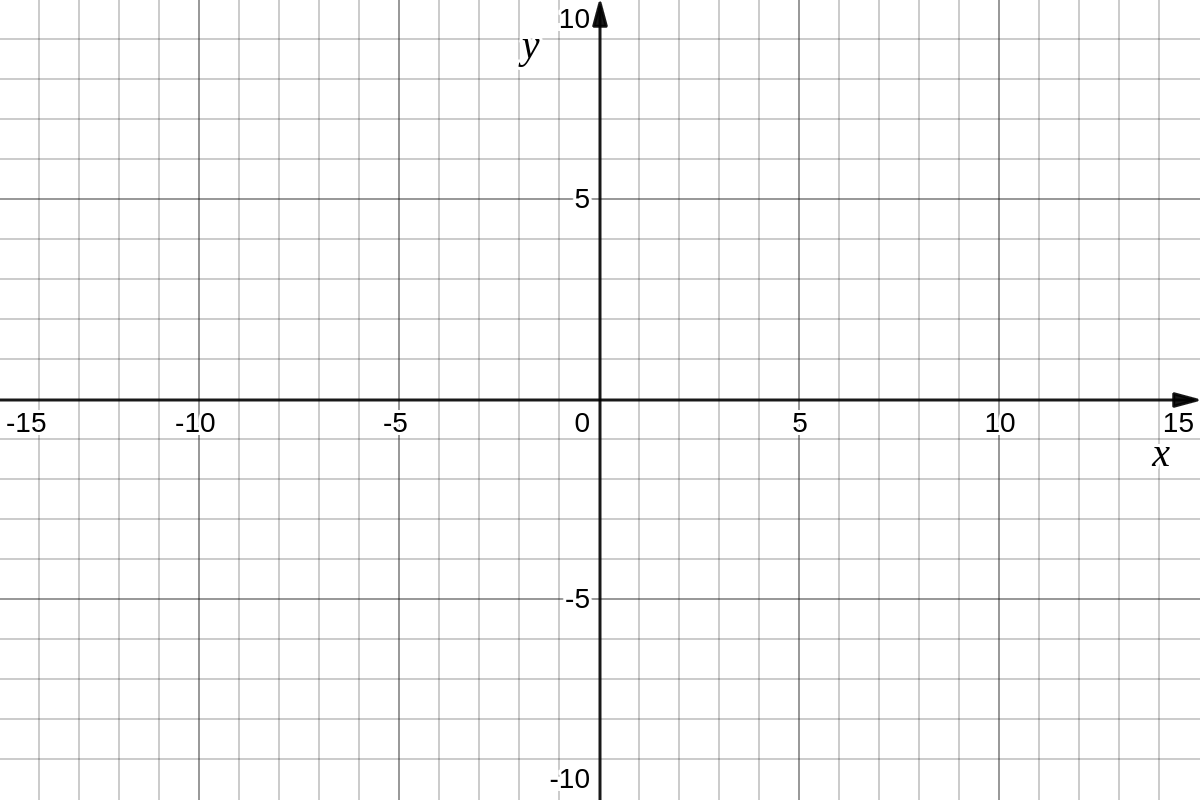
\includegraphics[width=.99\textwidth]{catesian.png}
\end{center}
\newpage
\section{Horizontal and Vertical Lines}
\subsection{Horizontal Lines}
Horizontal lines are express in the form \(y=a,\,a\in\mathbb R\).
\begin{center}
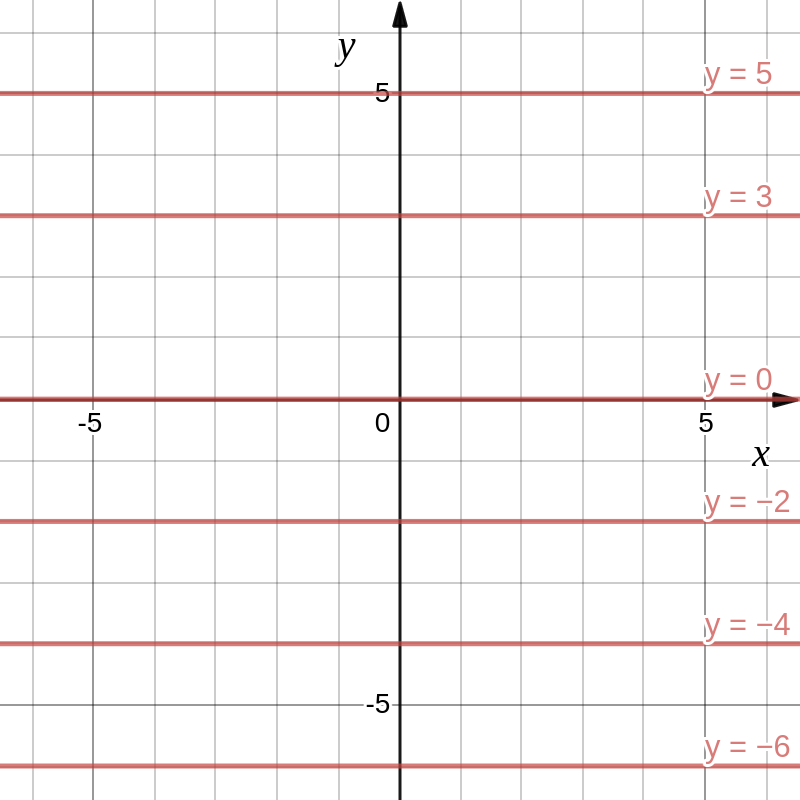
\includegraphics[width=.99\textwidth]{hori.png}
\end{center}
On the above diagram, draw the line \(y=2\).
\newpage
\subsection{Vertical Lines}
Vertical lines are express in the form \(x=b,\,b\in\mathbb R\).
\begin{center}
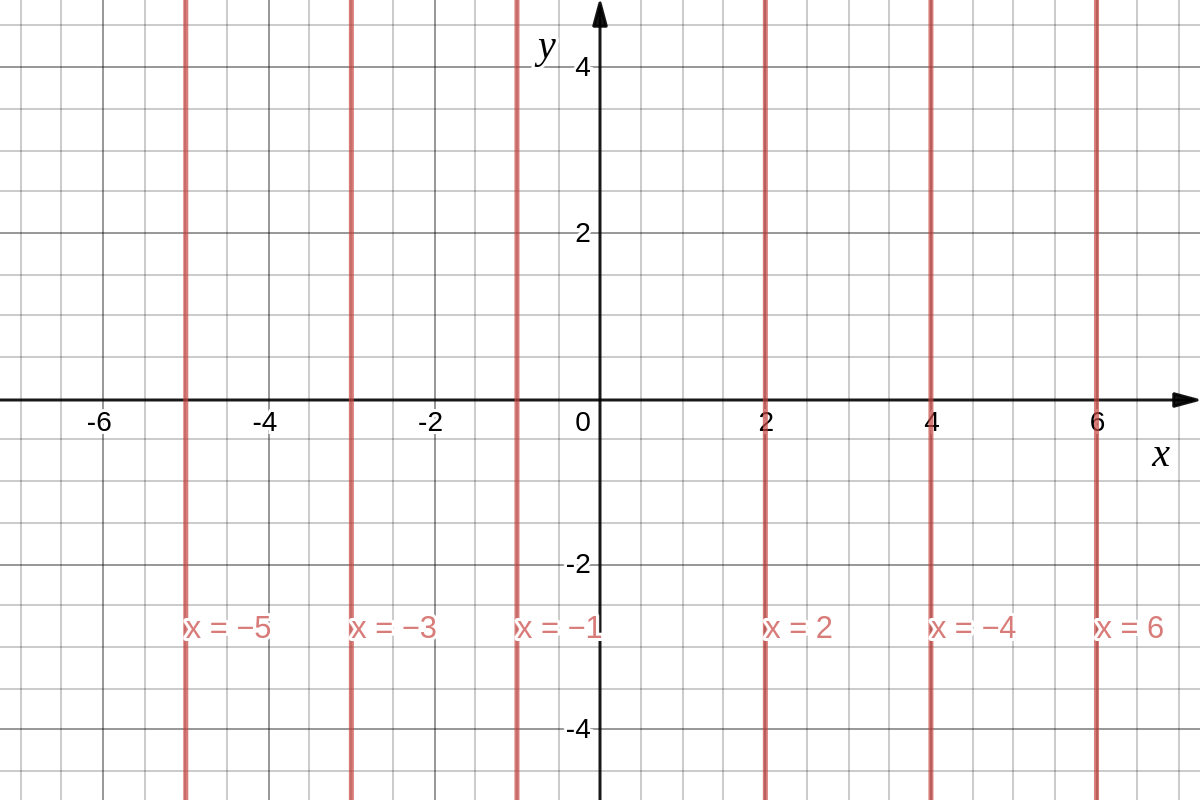
\includegraphics[width=.99\textwidth]{vert.png}
\end{center}
On the above diagram, draw the line \(x=1\).
\end{document}
